% コンパイル方法: lualatex filename.tex
\RequirePackage{plautopatch}

\documentclass[a4paper, 10pt]{ltjsarticle}


% マージン設定
\usepackage[top=20mm, bottom=20mm, left=20mm, right=20mm]{geometry}

% LuaLaTeX用日本語対応パッケージ
\usepackage{luatexja}
\usepackage{luatexja-fontspec}

% 必要なパッケージ
\usepackage{fontspec}
\usepackage{titlesec}
\usepackage{graphicx}
\usepackage{amsmath}
\usepackage{hyperref}
\usepackage[english, japanese]{babel}
\usepackage{multicol} % 二段組用パッケージ
\usepackage{indentfirst}
\usepackage{tikz} % カスタム点線用
\usepackage{authblk} % 著者・所属パッケージ
\usepackage{here}
\usepackage{caption}
\setmainfont[Ligatures=TeX]{Times New Roman}
\setmainjfont[BoldFont=MS Gothic]{MS Mincho}

\renewcommand{\baselinestretch}{0.95}

% セクション見出しのカスタマイズ
\titleformat{\section}
  {\fontsize{10pt}{10pt}}
  {\thesection.}
  {1em}{}


\setlength{\parindent}{1em}
% \setlength{\belowcaptionskip}{1em} % キャプション下の余白を -10pt に設定



\titlespacing*{\section}{0em}{1em}{0em}


\pagestyle{empty}


\begin{document}

\setlength{\columnsep}{7.5mm}

\twocolumn[
    \begin{center}
        {\vspace{-1em}}

        {\fontsize{15pt}{15pt}\selectfont{物理層からMAC層までの一貫したシミュレータ開発における\\CSMA/CAシミュレータの開発}}

        {\vspace{1.5em}}

        {\fontsize{13pt}{13pt}\selectfont{ Graduate Study Summary Format }}
    \end{center}



    % \vspace{-6.5em}

    \begin{flushright}
      {\fontsize{11pt}{11pt}\selectfont{T5-16 下沢亮太郎\\}}
      % \vspace{-0.2em}
      {\fontsize{11pt}{11pt}\selectfont{指導教員 設樂勇}}
    \end{flushright}

    \vspace{1em}

    \thispagestyle{empty}
]

\section{はじめに}

\section{従来手法}



\section{緒言}


\section{システムの概要}

BERTは、Googleによって開発された自然言語処理モデルであり、転移学習を行うことで特定のタスクに適応させることができる。

本研究では、大規模言語モデルを用いて作成した架空の企業ニュースと、それに応じた感情スコア(失望、楽観、懸念、興奮、安定の5つのパラメータ)を付与したデータセットを用いて、転移学習を行った。

転移学習後のBERTモデルの推論例を表1に示す。プラスの文章として「【速報】世界が注目するMVIDIAが決算発表『最終的な利益 前年比7。3倍2兆3300億円』勢い止まらず」、マイナスの文章として「UUスチール買収計画が窮地に 鉄鉄、訴訟も視野」という架空のニュースを用いた。プラスの文章では「楽観」と「興奮」、マイナスの文章では「懸念」と「失望」が高く出ており、期待した傾向を持つモデルを作成できたと考えられる。

BERTはGoogleが開発した自然言語処理モデルであり、転移学習により特定のタスクに適応可能である。

本研究では、大規模言語モデルで作成した架空の企業ニュースと、感情スコア(失望、楽観、懸念、興奮、安定)を付与したデータセットを用いてBERTの転移学習を実施した。






\section{システムの概要}

BERTは、Googleによって開発された自然言語処理モデルであり、転移学習を行うことで特定のタスクに適応させることができる。

本研究では、大規模言語モデルを用いて作成した架空の企業ニュースと、それに応じた感情スコア(失望、楽観、懸念、興奮、安定の5つのパラメータ)を付与したデータセットを用いて、転移学習を行った。

転移学習後のBERTモデルの推論例を表1に示す。プラスの文章として「【速報】世界が注目するMVIDIAが決算発表『最終的な利益 前年比7。3倍2兆3300億円』勢い止まらず」、マイナスの文章として「UUスチール買収計画が窮地に 鉄鉄、訴訟も視野」という架空のニュースを用いた。プラスの文章では「楽観」と「興奮」、マイナスの文章では「懸念」と「失望」が高く出ており、期待した傾向を持つモデルを作成できたと考えられる。

BERTはGoogleが開発した自然言語処理モデルであり、転移学習により特定のタスクに適応可能である。

本研究では、大規模言語モデルで作成した架空の企業ニュースと、感情スコア(失望、楽観、懸念、興奮、安定)を付与したデータセットを用いてBERTの転移学習を実施した。

% 推論例については表1に示す通り、「【速報】世界が注目するMVIDIAが決算発表『最終的な利益 前年比7.3倍2兆3300億円』勢い止まらず」というプラスの見出しにおいては「楽観」および「興奮」のスコアが高く、一方で「UUスチール買収計画が窮地に 鉄鉄、訴訟も視野」というマイナスの見出しにおいては「懸念」および「失望」のスコアが高く示された。これにより、モデルは期待される傾向に沿った結果を示したことが確認された。

% 元のやつ
% 表1にプラスの見出しとして「【速報】世界が注目するMVIDIAが決算発表『最終的な利益 前年比7.3倍2兆3300億円』勢い止まらず」、マイナスの見出しとしてUUスチール買収計画が窮地に 鉄鉄、訴訟も視野」を推論した結果を示した。プラスの見出しでは楽観と「興奮」が高く、マイナスの見出しでは「懸念」と「失望」が高く出たため、モデルは期待通りの傾向を示した。

% アディ
表1に二つの見出しの例を示した。
プラスな印象を受ける見出しとして、「【速報】世界が注目するMVIDIAが決算発表『最終的な利益 前年比7.3倍2兆3300億円』勢い止まらず」、
マイナスな印象を受ける見出しとして「UUスチール買収計画が窮地に 鉄鉄、訴訟も視野」を推論した結果を示した。
プラスの見出しでは楽観と「興奮」が高く、マイナスの見出しでは「懸念」と「失望」が高く出たため、モデルは期待通りの傾向を示した。

% 推論例として、表1に「【速報】世界が注目するMVIDIAが決算発表『最終的な利益 前年比7.3倍2兆3300億円』勢い止まらず」というプラスの見出しでは「楽観」と「興奮」が高く、「UUスチール買収計画が窮地に 鉄鉄、訴訟も視野」というマイナスの見出しでは「懸念」と「失望」が高く出たため、モデルは期待通りの傾向を示した。



\begin{table}[h]
    \centering
    \caption{推論結果例}
    \vspace{-0.5em}
    \begin{tabular}{|c|c|c|c|c|}\hline
        \multicolumn{5}{|c|}{プラスの文章} \\ \hline
        失望 & 楽観 & 懸念 & 興奮 & 安定 \\ \hline
        0.0534 & 0.395 & 0.109 & 0.231 & 0.212 \\ \hline
        \multicolumn{5}{|c|}{マイナスの文章} \\ \hline
        失望 & 楽観 & 懸念 & 興奮 & 安定 \\ \hline
        0.254 & 0.110 & 0.351 & 0.135 & 0.150 \\ \hline
    \end{tabular}

\end{table}

また、LSTMの説明変数として5つの感情パラメータの他にNASDAQ100指数、S\&P500指数、恐怖指数を採用し、目的変数を各株式の一日の終値とした。

図1にシステム全体の概要図を示す。

% \begin{figure}[H]
%     \centering
%     \includegraphics[width=0.65\columnwidth]{./assets/system.png}
%     \caption{システム全体の概要図}
% \end{figure}



\section{結果}

% 約500社を1社ごとに学習したモデルのMAE(Mean Absolute Error)の分布を以下に示す。test\_maeの中央値が0.059となり、良い値に見えるがデータの量が少なく過学習気味になっていることやデータを収集していた時期は全体的に上昇気味だったことに注意が必要である。

% 元
% 約500社のスクレイプしたデータを個別に学習したモデルのMAE(Mean Absolute Error)の分布を図2に示す。test\_maeの中央値は0.059と良好に見えるが、データ量が少なく過学習の可能性や、データ収集時期が全体的に上昇傾向だった点に注意が必要である。

ウェブスクレイピングにより取得した約500社データを個別に学習したモデルのMAE(Mean Absolute Error)の分布を図2に示す。\texttt{test\_mae}の中央値は0.059と良好に見えるが、これはデータ不足による過学習やデータ収集時期が全体的に上昇傾向だったことに起因すると考える。



% \begin{figure}[H]
%     \centering
%     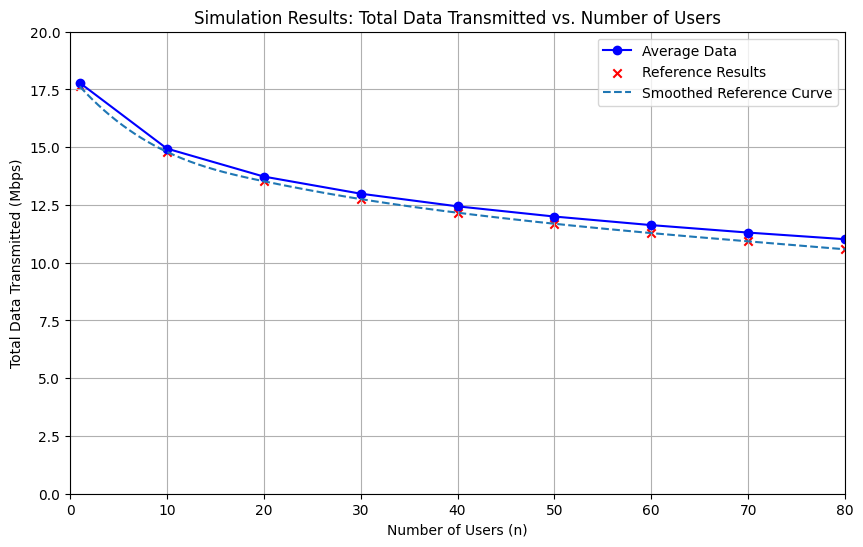
\includegraphics[width=0.9\columnwidth]{./assets/graph.png}
%     \caption{MAEの分布}
% \end{figure}

\section{結言}

本研究では、ニュースから得られる感情情報を活用し、株価推移を予測するシステムを構築した。今後は、評価方法の改善等を通じて、実用化を目指す。

% 本研究では、ニュースの感情情報を活用して株価推移を予測するシステムを構築した。今後は評価方法の改善を進め、実用化を目指す。
% 本研究では、ニュースの感情情報を活用して株価推移を予測するシステムを構築した。


% カスタム点線を描画
\noindent
\begin{tikzpicture}
\draw[dotted, thick] (0, 0) -- (\linewidth, 0);
\end{tikzpicture}

お問い合わせ先\\
氏名:高田 拓 \\
E-mail : \href{mailto:takada@metro-cit.ac.jp}{takada@metro-cit.ac.jp}

\end{document}
